%!TeX root =  ../../thesis.tex

\section{Klíčové třídy}
\subsection{Controller}
Controller, jak název napovídá, je hlavní třída, která řídí běh zařízení a ačkoliv hlavní část je v code.ino, třída Controller zpřehlední kód, jelikož podléhá standardnímu zápisu C++ kódu. Třída Controller obsahuje dvě důležité veřejné metody a to metodu \hl{run()} a \hl{initialize()}.

\subsubsection{Metoda initilize()}
Tato metoda inicializuje zařízení a volá metody pro inicializaci na komponentech, v případě, že nastane chyba, zařízení se jí pokusí ohlásit, výpisem na displej a zvukovým signálem, v intervalu SOS v morseovce. Tato metoda je volána v metodě \hl{setup()} při přípravě zařízení a na jejím konci se při úspěchu ozve bzučák s krátkým pípnutím, které oznámí, že zařízení je připravené k použití.

\subsubsection{Metoda run()}
Tato metoda hlavní činnost programu pro tester a je volána v metodě \hl{loop()}. Na začátku metody se zkontroluje vstup z klávesnice, pokud nějaký je, tak se vykoná příslušná akce, pak se řeší probliknutí kontrolního znaku na displeji.

\subsection{Connector}
Třída Connector slouží jako předek pro konkrétní konektory, ačkoliv není abstraktní a dá se vytvořit instance, tak dědění nám zpřehledňuje kód, už jen kvůli tomu, že vždy nemusíme vyplnit celý její konstruktor, který si žádá mnoho parametrů, jako jsou například název, pole s čísly příslušných pinů, odkaz na proti konektor a atp.. Tato třída obsahuje také společné metody pro práci s konektory, které si nyní popíšeme.

\subsubsection{void setMode(Mode mode)}
Na obrázku \ref{fig:setMode} je implementace metody, která nastavuje piny, na které je konektor připojen, na vstupní nebo výstupní.  Rozhoduje pomocí hodnoty parametru, kterým je enumerátor Mode. Použití enumerátoru dělá kód přehlednější a dá se s ním lépe pracovat oproti aliasům na režimy definované v \hl{Arduino.h}. Enumerátor Mode je také atributem třídy Connector a tato metoda slouží zároveň jako setter pro tento atribut.

\begin{figure}[H]
	\centering
	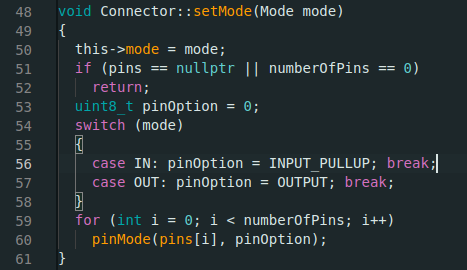
\includegraphics[width=0.9\textwidth]{pictures/setMode.png}
    	\caption{Metoda setMode(Mode)}
   	\label{fig:setMode}
\end{figure}

Metoda je ošetřena proti chybám, ze jména pak proti nulovému ukazateli na pole s čísly pinů. Ačkoliv by se dalo pracovat pouze s číselnou hodnotou aliasů, jak je patrné z implementace, tak enumerátor, jak již bylo zmíněno, dělá kód přehlednější, jelikož například \hl{bosh.setMode(Mode:IN);} je samovysvětlující oproti \hl{bosh.setMode(2);}.

\subsubsection{void reconnectTo(Connector* connector)}
Metoda reconnectTo(Connector*) nastavuje ukazatel na protější konektor a vytváří název spojení, který se bude zobrazovat v menu.

\begin{figure}[H]
	\centering
	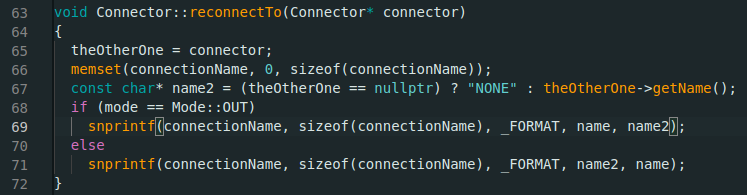
\includegraphics[width=0.9\textwidth]{pictures/reconnect.png}
    	\caption{Metoda reconnectTo(Connector*)}
   	\label{fig:reccon}
\end{figure}

Implementace metody na obrázku \ref{fig:reccon} ukazuje, že neslouží jako setter na ukazatel na instanci objektu protějšího konektoru, ale také nastaví/přenastaví jméno spojení, aby bylo bylo možné jej zobrazit v menu, tak, že výstupní konektor je vpravo, tudíž výsledný formát je například \hl{Xlr3~\texttt{->}~Jack 2.1}.

\subsubsection{bool startTest(char resultArr[])}
Toto je metoda na spuštění testu, jako parametr bere pole znaků, ačkoliv se nejedná o textový řetězec, ale o pole s malými čísly. Na první místo se píše stav testu, hodnota 0 je pro úspěšný test a záporné jsou pro chyby. Zbytek pole pak obsahuje buď -100 nebo číslo pinu na konektoru, který je vadný. V případě úspěšného testu je návratová hodnota \textbf{true}, jinak vždy \textbf{false}. Tato metoda také kontroluje, zda-li je test proveditelný. Mezi kontrolované případy patří: nulový ukazatel na protější konektor, špatně nastavený konektor nebo že oba jsou výstupní nebo vstupní. Metodu, která provádí samotné testování popíši v kapitole Testování.

\subsection{IComponent}
Společný předek pro komponenty zařízení, jako jsou například: displej, klávesnice nebo bzučák. Tento předek obsahuje jednu čistě virtuální funkci a to funkci \hl{inicialize()}, která vrací \textbf{true}, když se podaří danou komponentu inicializovat.
